\mcchap{Manuale utente}{cap:manuale}

\section{Esecuzione in locale}

\subsection{Requisiti software}
Il progetto è stato realizzato utilizzando \emph{ambiente di sviluppo integrato} (IDE) Pycharm Community.
Per l'esecuzione della dashboard sono richieste le seguenti dipendenze.
\begin{itemize}
 \item Git
 \item Python 3.8.5
 \item Pandas
 \item Plotly 
 \item Dash 
 \item Dash Bootstrap Components
 \end{itemize}
 
 \subsection{Clonazione del repository}
 E' possibile scaricare il progetto direttamente dal mio repository Github, con il comando \texttt{git clone https://github.com/alex27riva/Covid-dashboard}
 
 \subsection{Installazione dipendenze}
 Per installare le librerie richieste è sufficiente lanciare i seguenti comandi dal termianle integrato in Pycharm.
 
 \begin{itemize}
     \item \texttt{\$ pip install pandas}
     \item \texttt{\$ pip install plotly==4.12.0}
     \item \texttt{\$ pip install dash==1.17.0}
     \item \texttt{\$ pip install dash-bootstrap-components}
 \end{itemize}
 
 \begin{figure}[htp]
    \centering
    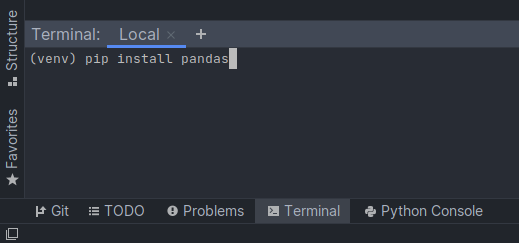
\includegraphics[width=10cm]{pycharm_terminal}
    \caption{Terminale integrato in Pycharm}
    \label{fig:pycharm_termianl}
\end{figure}

Ad installazione completata, sarà possibile avviare il progetto.

\subsection{Avvio del programma}
Per l'avvio del programma, cliccare sul pulsante con la freccina verde (nella figura \ref{fig:run_dash}.
\begin{figure}[htp]
    \centering
    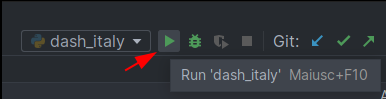
\includegraphics[width=8cm]{img/run_dash.png}
    \caption{Avvio del programma}
    \label{fig:run_dash}
\end{figure}
Verrà avviato un server locale, il cui suo URL verrà mostrato nella console di debug a cui si potrà visualizzare la pagina della dashboard.

 \begin{figure}[htp]
    \centering
    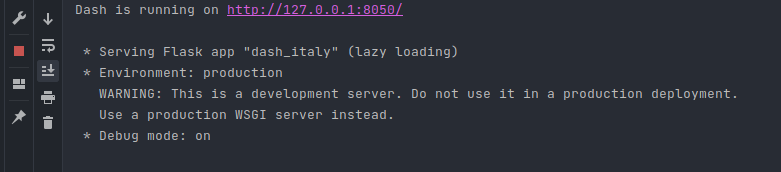
\includegraphics[width=9cm]{running_program}
    \caption{Programma Python in esecuzione}
    \label{fig:running_program}
\end{figure}

\section{Configurazione della VPS}
E' necessario disporrre di un server privato virtuale (VPS) con sistema operativo Ubuntu Server.

\subsection{Creazione account utente}
Per questioni di sicurezza è meglio non utilizzare l'account privilegiato \emph{root}.
\begin{enumerate}
\item Collegarsi alla VPS tramite SSH \texttt{ssh root@<ip-della-VPS>}
\item Crea l'account per l'utente admin \texttt{useradd -m admin}
\item Imposta una password per l'utente admin \texttt{passwd admin}
\item Chiudi la connessione con il comando \texttt{exit}
\end{enumerate}

\subsection{Installazione di Docker}

\begin{enumerate}
\item Collegarsi alla VPS con l'account admin \texttt{ssh admin@<ip-della-VPS>}
\item Scaricare lo script per l'installazione di Docker \texttt{curl -fsSL https://get.docker.com -o get-docker.sh}
\item Eseguire lo script con \texttt{sudo sh get-docker.sh}
\item Eseguire questo comando per interagire con Docker senza previlegi di root \texttt{sudo usermod -aG docker admin}
\end{enumerate}

\subsection{Installazione e avvio dei container}
I container con le tre dashboard sono presenti nei repository di Docker, è sufficiente eseguire i seguenti comandi per la loro installazione e avvio.
\begin{itemize}
\item \texttt{docker run -d -p 8050:8050 --name=dash\_italy alex27riva/dash\_italy}
\item \texttt{docker run -d -p 8051:8050 --name=dash\_lomb alex27riva/dashboard\_lombardia}
\item \texttt{docker run -d -p 8052:8050 --name=dash\_regioni alex27riva/dashboard\_regioni}
\end{itemize}

\subsection{Portainer}
Per una gestione più semplice dei container Docker è possibile installare Portainer, un interfaccia web che facilita l'avvio, aggiornamento, rimozione dei container.
Per installare Portainer sono necessari questi due comandi:
\begin{enumerate}
    \item \texttt{docker volume create portainer\_data}
    \item \texttt{docker run -d -p 8000:8000 -p 9000:9000 --name=portainer --restart=always\\ -v /var/run/docker.sock:/var/run/docker.sock -v portainer\_data:/data\\ portainer/portainer-ce}
\end{enumerate}
Ora ci si può collegare all'interfaccia web all'indirizzo \emph{http://\textless ip-vps\textgreater:9000}

\subsection{Ngnix}
Ngnix è un web server, che è stato utilizzato come reverse proxy.
\subsubsection*{Installazione di Ngnix}

\begin{enumerate}
    \item \texttt{sudo apt update}
    \item \texttt{sudo apt install nginx}
    \item \texttt{unlink /etc/nginx/sites-enabled/default}
    \item \texttt{sudo nano /etc/nginx/sites-available/reverse-proxy.conf}
\end{enumerate}

\begin{lstlisting}[basicstyle=\ttfamily\small]
server
 {
    listen 80;
    listen 443;
    listen [::]:80;
    ssl on;
    ssl_certificate /etc/letsencrypt/live/dash.covid19-italy.it/fullchain.pem;
    ssl_certificate_key /etc/letsencrypt/live/dash.covid19-italy.it/privkey.pem;

    server_name dash.covid19-italy.it
    
    access_log /var/log/nginx/reverse-access.log;
    error_log /var/log/nginx/reverse-error.log;
    
    location /italy/ {
                proxy_pass http://localhost:8050;

    }

    location /lombardy/ {
            proxy_pass http://localhost:8051;

    }

    location /regions/ {
            proxy_pass http://localhost:8052;

    }
}
\end{lstlisting}

\subsubsection*{Creazione del link simbolico}
\texttt{\$ ln -s /etc/nginx/sites-available/reverse-proxy.conf\\ /etc/nginx/sites-enabled/reverse-proxy.conf}

\subsubsection*{Test della configurazione}
\texttt{nginx -t}

\subsection{Installazione certificato SSL}
\begin{enumerate}
\item Assicurarsi che snap sia aggiornato \texttt{sudo snap install core; sudo snap refresh core}
\item Installare Certbot \texttt{sudo snap install --classic certbot}
\item Crea link simbolico per l'eseguibile \texttt{sudo ln -s /snap/bin/certbot /usr/bin/certbot}
\item Richiesta del certificato \texttt{sudo certbot --nginx}
\end{enumerate}

\subsection*{Riavvio di Nginx}
Riavviare il servizio di Nginx con il seguente comando: \\
\texttt{sudo systemctl restart nginx}

